%!TEX root = fourier.tex


\chapter{Transformée de Fourier}

%\begin{remark}[\textbf{Erratum sur le chapitre \emph{Séries de Fourier}}]

%Dans le paragraphe~\ref{cours-parseval} sur Parseval, le coefficient
%$a_0$ doit être remplacé par $a_0^2$ :
%
%Une propriété importante des séries de Fourier est le théorème de
%Parseval. Soit une fonction $f$, périodique de période $T$. Dans les
%cas des coefficients complexes et réels, l'égalité de Parseval s'écrit
%:

%\begin{equation}
%a_0^2+\frac{1}{2}\sum_{n=1}^\infty (a_n^2+b_n^2)=\quad \sum_{n=-\infty}^\infty | c_n|^2 \quad=\quad \frac{1}{T}\int_{periode~T}|f(x)|^2 dx
%\end{equation}

%Une interprétation de cette propriété est que l'énergie du signal sur
%la période est la même, qu'elle soit mesurée dans le domaine {
%direct } $x$ (temporel, souvent), ou dans le domaine de Fourier.

%Un point pratique qui découle de cette expression est que les sommes
% $a_0^2 + \frac{1}{2}\sum_{n=1}^\infty (a_n^2+b_n^2)$ et
% $\sum_{n=-\infty}^\infty | c_n|^2 $ sont convergentes, ce qui
% implique que les coefficients de Fourier doivent décroître
% suffisamment vite en fonction de $n$. Si vos calculs aboutissent à
% des coefficients qui décroissent trop lentement avec $n$, voire
% augmentent, c'est qu'il faut faire la chasse aux erreurs...

%\end{remark}

\section{Définition de la transformée de Fourier}

\begin{remark}

Beaucoup d'enseignants et de livres utilisent indifféremment (et
parfois sans souci d'homogénéité) $i$ ou $j$ pour noter le complexe
dont le carré vaut -1. \`A part s'habituer, pas de remède...

\end{remark}

\begin{definition}
Une fonction $f$ est dite absolument intégrable si $\inttotal |f(t)|dt<\infty$. \\ On note généralement $L^1(\RR)$ l'ensemble de ces fonctions.


\end{definition}


%%%%%%%%%%%%%%%%%%%%%%%%%%%%%%%%%%%%%%%%%%%%%%%%%%%%%%%%%%%%%%%%
\begin{boxedminipage}{15cm}
\begin{definition}

Si $f$ est une fonction absolument intégrable, elle admet une transformée de Fourier, notée de diverses manières : $\BF(f)=TF(f)=F$, et définie par :
\begin{equation}
{\bf F(\om)=\inttotal f(t)e^{-j\om t}dt}
\end{equation}

Transformation de Fourier inverse :

 \begin{equation}
{\bf f(t)=\frac{1}{2\pi}\inttotal F(\om)e^{j\om t}d\om}
\label{reconstruction}
\end{equation}

\begin{remark}
Aux (éventuels) points de discontinuités de $f$, l'expression~\ref{reconstruction} est à remplacer par : 
 \begin{equation}
\frac{1}{2\pi}\inttotal F(\om)e^{j\om t}d\om=\frac{f(t^-)+f(t^+)}{2}
\label{reconstruction2}
\end{equation}
(moyenne des limites à gauche et à droite)
\end{remark}
\end{definition}
\end{boxedminipage}
%%%%%%%%%%%%%%%%%%%%%%%%%%%%%%%%%%%%%%%%%%%%%%%%%%%%%%%%%%%%%%%%%%%%%%%%

\begin{example}
\label{ex_rectangle}

Soit la fonction :
\begin{eqnarray}
    f(t)=
\begin{cases}
  1   & \text{si}~ |t|<\frac{a}{2} \quad (a>0, \quad \text{constante}) \\
  0 & \text{sinon} 
\end{cases}
\end{eqnarray}

On peut montrer que sa transformée de Fourier est 
\begin{equation}
F(\omega)= a.sinc(\frac{\omega.a}{2}) \quad \text{où} \quad sinc(x)=\frac{sin(x)}{x}
\end{equation}

Le recours à la "notation-fonction" $sinc$ est facultatif.

\begin{figure}{H}
\begin{center}
\begin{tikzpicture}[background rectangle/.style={fill=olive!5}, show background rectangle]
\begin{groupplot}[group style={group size=1 by 2, horizontal sep=2cm, vertical sep=2cm},scale=0.7,samples=150]
\nextgroupplot[title={$f(t)$}]
\addplot[blue,ultra thick,domain=-2:-0.5]{0};
\addplot[blue,ultra thick,domain=-0.5:0.5]{1};
\addplot[blue,ultra thick,domain=0.5:2]{0};
\nextgroupplot[title={$F(\omega)$}]
\addplot[blue,ultra thick,domain=-15:15]{2*sin(deg(x/2))/x};
\end{groupplot}
\end{tikzpicture}
\hspace*{2cm}
\begin{tikzpicture}[background rectangle/.style={fill=olive!5}, show background rectangle]
\begin{groupplot}[group style={group size=1 by 2, horizontal sep=2cm, vertical sep=2cm},scale=0.7,samples=150]
\nextgroupplot[title={$f(t)$}]
\addplot[blue,ultra thick,domain=-2:-1]{0};
\addplot[blue,ultra thick,domain=-1:1]{1};
\addplot[blue,ultra thick,domain=1:2]{0};
\nextgroupplot[title={$F(\omega)$}]
\addplot[blue,ultra thick,domain=-15:15]{sin(deg(x))/x)};
\end{groupplot}
\end{tikzpicture}
%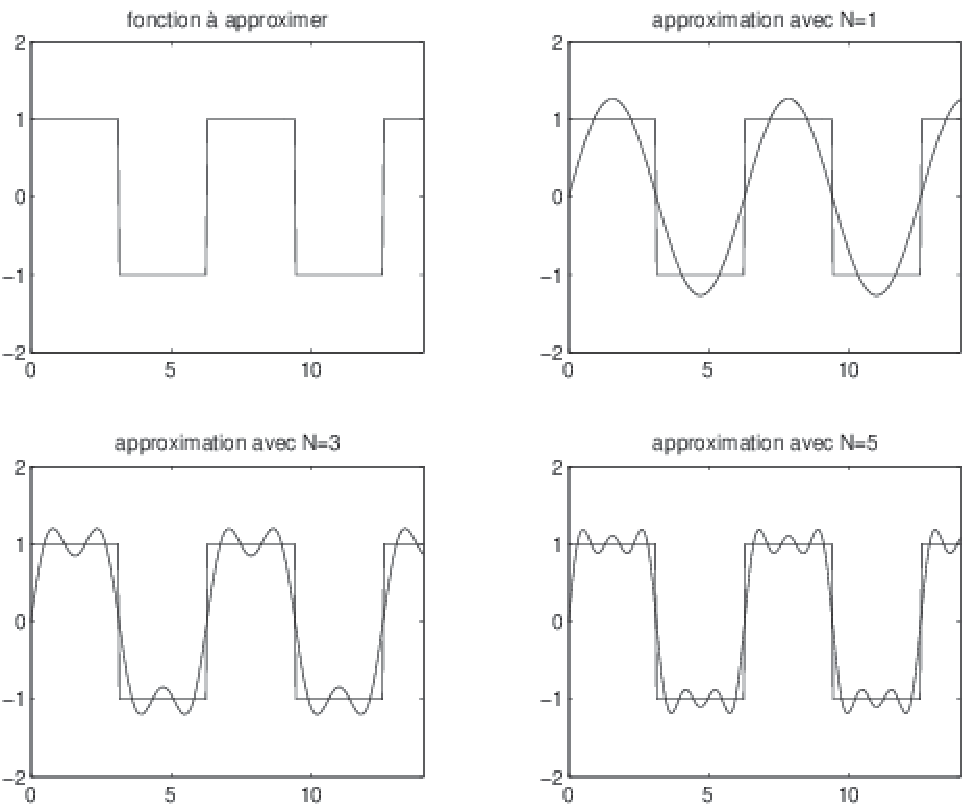
\includegraphics[scale=0.63]{reconstruction.pdf}
\caption{Transformée de Fourier d'une fonction "fenêtre". Les deux colonnes sont deux exemples ($a=1$ et $a=2$) du cas général de l'exemple \ref{ex_rectangle}. Les abscisses sont en radians.}
\end{center}
\label{fourier_transform_example}
\end{figure}

Le réel $a$ est ici un paramètre réglant la largeur de la porte, et la
transformée de Fourier de $f$ sera bien sûr fonction de $a$. Ceci
permettra de s'interroger sur la manière dont varie la transformée
quand on fait varier la largeur de la porte.  Cet exemple a une grande
importance dans les applications et mérite d'être mémorisé. %On le
retrouvera dans le chapitre sur l'analyse temps-fréquence.

\end{example}

%{\footnotesize
\begin{remark}[De la diversité des définitions (pas très important)]

Vous pourrez rencontrer, dans certaines sources d'information,
d'autres définitions de la transformée de Fourier et de la transformée
inverse, qui ne changent qu'à un facteur constant près, notamment :
\begin{equation}
F(\om)=\frac{1}{\sqrt{2\pi}}\inttotal f(t)e^{-j\om t}dt
\end{equation}
 \begin{equation}
f(t)=\frac{1}{\sqrt{2\pi}}\inttotal F(\om)e^{j\om t}d\om
\end{equation}

\end{remark}

\begin{definition}
Une fonction $f$ est dite à énergie finie (\emph{square-integrable} en anglais a le mérite de la clarté) si $\inttotal |f(t)|^2dt<\infty$. \\ On note généralement $L^2(\RR)$ l'ensemble de ces fonctions.
\end{definition}


\section{Propriétés de la transformée de Fourier}

On retrouve ici des propriétés qui étaient généralement déjà vraies et vues pour les séries de Fourier.
Pour la plupart d'entre elles, la démonstration est assez facile et un bon exercice.

\subsection{Expressions alternatives de la transformée dans des cas particuliers}

Dans les cas suivants, les simplifications obtenues n'empêchent pas
d'utiliser l'expression { standard }~\ref{reconstruction}, qui
reste parfois préférable pour la simplicité du calcul.

\begin{equation}
\text{Si $f$ est paire} \quad F(\om)=2\intpositive f(t)cos(\om t)dt
\end{equation}

 \begin{equation}
\text{Si $f$ est impaire} \quad F(\om)=-2j\intpositive f(t)sin(\om t)dt    
  \end{equation}
\subsection{Linéarité}

Soient $f$ et $g$ deux fonctions admettant une transformée de Fourier et $\lambda$ et $\mu$ deux réels. La transformée de Fourier de la combinaison linéaire est la combinaison linéaire des transformées de Fourier.
\begin{equation} \label{transfo-linearite}
\quad \BF(\lambda f+\mu g)=\lambda \BF(f)+\mu \BF(g)
\end{equation}

Un intérêt est que la transformée de Fourier d'une fonction qui n'est pas simple, mais qui peut s'exprimer comme la combinaison linéaire de fonctions élémentaires, peut être calculée par la combinaison linéaire des transformées de Fourier de ces fonctions élémentaires.

%\text{c'est-à-dire :} \quad $\BF(\lambda f+\mu g)(\omega)=\lambda \BF(f)(\omega)+\mu \BF(g)(\omega)$

\subsection{Dérivation}
Si $f'$ est la dérivée de $f$ et si elle admet une transformée de Fourier alors :
\begin{equation} \label{transfo-derivation}
  \BF(f')(\om)=j\om \BF(f)(\om)
\end{equation}


\subsection{Translation temporelle}
\label{signalretard}
Notons $f_\tau$ la fonction telle que $f_\tau(t) = f(t-\tau)$.
%
On peut montrer facilement que :
\begin{equation} \label{transfo-translation}
\BF(f_\tau)(\om)=e^{-j\om\tau} \BF(f)(\om)
\end{equation}
En particulier, remarquons que, conformément à l'intuition, la translation temporelle d'un signal ne change pas la répartition de son énergie sur l'ensemble des fréquences, mais n'affecte que la phase de la transformée :
\begin{equation}
|\BF(f_\tau)|=|\BF(f)|
\end{equation}

C'est une bonne occasion de se rappeler que le spectre fréquentiel
d'un signal, que l'on trace et que l'on interprète assez
familièrement, omet l'information de phase. Celle-ci n'en est pas pas
moins essentielle à la reconstruction du signal dans le domaine
temporel, et $F(\om)$, qui apparait dans le calcul de la transformée
inverse, est, de manière générale, une quantité complexe.

Cette propriété s'appelle parfois { théorème du retard }.  Vous
pourriez examiner et tenter d'interpréter l'effet, dans le domaine
temporel, d'une translation réalisée dans le domaine de Fourier.

\subsection{Homothétie}
Pour une réel $k>0$,
\begin{equation}
 \BF(f(kt)))=\frac{1}{k}\BF(f(\frac{t}{k}))
\end{equation}

Un cas assez simple d'application particulière, qui recoupe une situation déjà traitée, est la fonction porte de largeur quelconque.

\subsection{Égalité de Parseval}

Comme dans le cas des séries de Fourier, cette égalité établit l'égalité de l'énergie vue dans le domaine d'origine ({ temporel }) et le domaine de Fourier ({ fréquentiel }).

\begin{equation}
  \label{eq:parseval2}
  \inttotal |f(t)|^2dt=\frac{1}{2\pi}\inttotal|F(\om)|^2d\om
\end{equation}
Attention, de façon générale, il s'agit de modules sur des complexes et pas seulement de valeurs absolues apparemment superflues.

\section{Convolution, Dirac et Transformée de Fourier}

Il est utile de voir 
\begin{equation}
(f*g)(t)=\inttotal f(\tau)g(t-\tau)d\tau
\end{equation}
comme un produit scalaire entre fonctions.

La convolution est une opération qui combine deux fonctions $f$ et $g$ pour en créer une troisième, notée $f*g$. Souvent, dans les applications, $f$ est un signal et $g$ est un filtre (ou noyau)  que la convolution vient appliquer sur le signal $f$ pour l'améliorer ou en tirer une information intéressante. La convolution est aussi impliquée dans la construction de représentation de séquences ou d'images pour faire de l'apprentissage et de la reconnaissance.

Imaginons qu'un phénomène qui nous intéresse produit un signal $f(t)$ où $t$ désigne le temps, au fond de l'espace lointain. Pas de chance : comme ce signal nous vient de loin dans l'espace, ce long voyage lui fait subir des perturbations. Pour 

\begin{boxedminipage}{15cm}
\begin{definition}
Soient $f$ et $g$ deux fonctions à énergie finie.
%Soit $h(t)$ le 
Le produit de convolution entre $f$ et $g$ noté $f*g$ est défini par :

%(on note souvent $h=f*g$ ou $h(t)=(f*g)(t)$) :
\begin{equation}
(f*g)(t)=\inttotal g(\tau)f(t-\tau)d\tau
\end{equation}
\end{definition}
\end{boxedminipage}

\newcommand{\convscale}{0.52}

\begin{figure}
\begin{center}
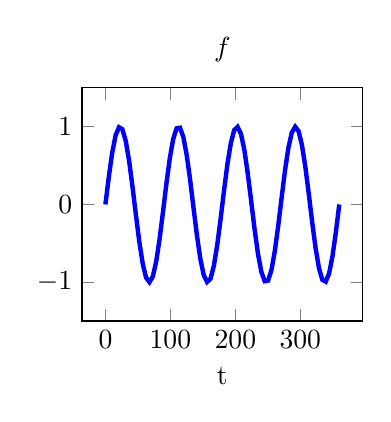
\begin{tikzpicture}
\begin{axis}[scale=\convscale,ymin=-1.5,ymax=1.5,samples=70, xlabel={t},title={$f$}]
 \addplot[domain=0:360, blue,  ultra thick]{sin(4*x)};
\end{axis}
\end{tikzpicture}
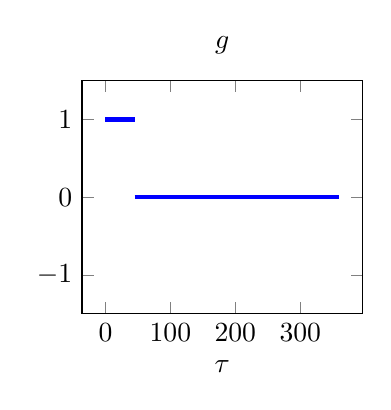
\begin{tikzpicture}
\begin{axis}[scale=\convscale,ymin=-1.5,ymax=1.5,xlabel={$\tau$},title={$g$}]
 \addplot[domain=0:45, blue,  ultra thick]{1};
 \addplot[domain=45:360, blue,  ultra thick]{0};
\end{axis}
\end{tikzpicture}
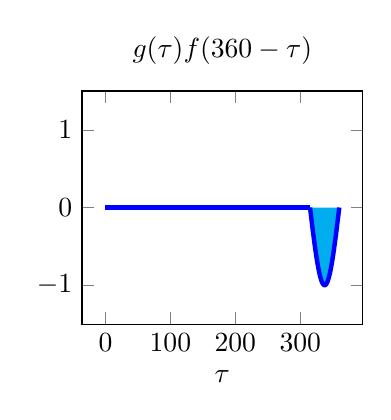
\begin{tikzpicture}
\begin{axis}[scale=\convscale,ymin=-1.5,ymax=1.5,samples=70, xlabel={$\tau$},title={$g(\tau)f(360-\tau)$}]
  \addplot[domain=0:315, blue,  ultra thick]{0};
  \addplot[domain=315:360, blue, fill=cyan, ultra thick]{sin(4*x)};
\end{axis}
\end{tikzpicture}
\end{center}
\caption{Illustration d'une étape de la convolution. Cas particulier de $t=360$}
\end{figure}

Le produit de convolution vérifie :
\begin{eqnarray}
  f*g & =g*f & \textit{(commutativité)} \label{convolution-commut}\\
\text{~donc~} (f*g)(t) &=\inttotal f(t-\tau)g(\tau)d\tau & \\
f*(g+h) & =f*g+f*h & \textit{(distributivité)} \label{convolution-distrib}\\
(f*g)' & =f'*g=f*g' & \textit{(dérivation)} \label{convolution-derivation}
\end{eqnarray}

Il possède une propriété importante concernant la transformation de Fourier :

\begin{equation} \label{convol_transfo1}
\BF(f*g)=\BF(f).\BF(g)
\end{equation}
et dans le sens inverse :
\begin{equation}
  \BF(f.g)=\frac{1}{2\pi}\BF(f)*\BF(g)
\end{equation}

La même propriété existe d'ailleurs pour les séries de Fourier :
\begin{equation}
c_n(f*g)=c_n(f).c_n(g)
\end{equation}

Pour s'en tenir à un point de vue très pratique, la convolution donne un moyen parfois astucieux de calculer (manuellement) des transformées de Fourier de fonctions que l'on parvient à identifier comme produit de convolution de deux fonctions assez simples. 
Plus largement que le calcul de transformée, si on doit réaliser la convolution d'un signal par un filtre linéaire (par exemple filtrer un son ou une image), l'opération peut être réalisée dans le domaine de Fourier par une multiplication, ce qui permet parfois de réduire considérablement le coût (informatique) de calcul.

\begin{example}
L'exercice où on voit que la convolution d'une fonction { porte
} par elle-même donne un triangle est l'occasion d'aller creuser un
peu : le triangle est plus { lisse } que la porte (il est déjà continu,
à défaut d'être dérivable). Convoluons ce triangle par lui-même, et ce
résultat par lui-même, etc. pour voir vers quoi cela semble converger
:

\begin{center}
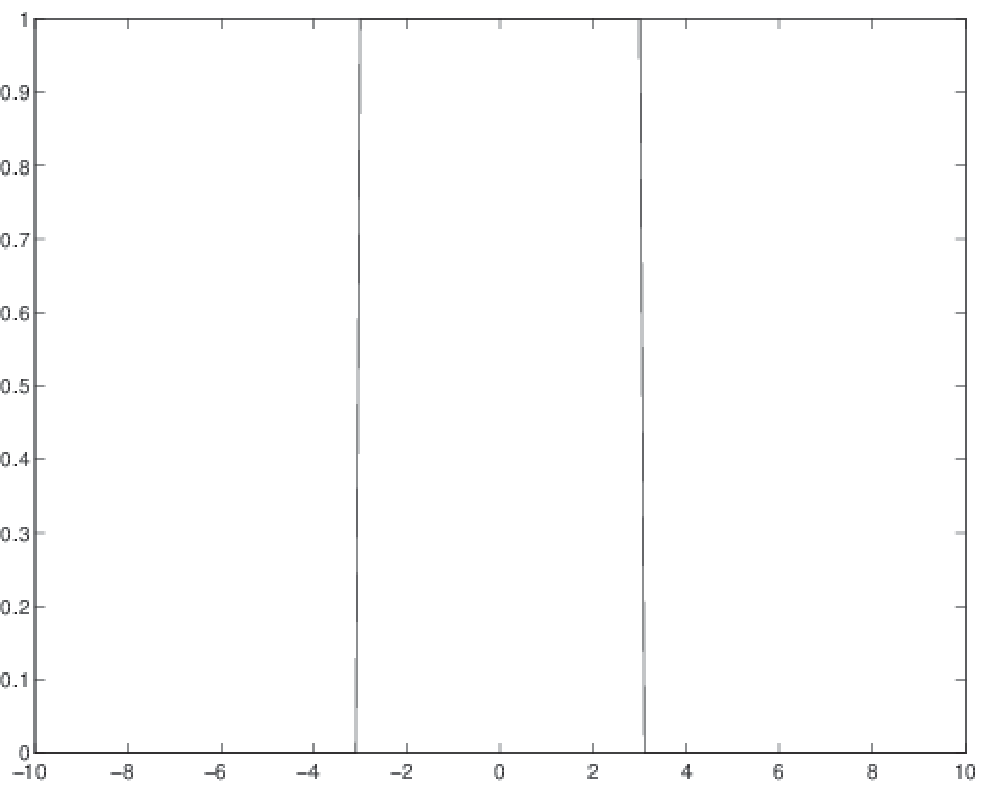
\includegraphics[scale=0.25]{convgauss1.pdf} 
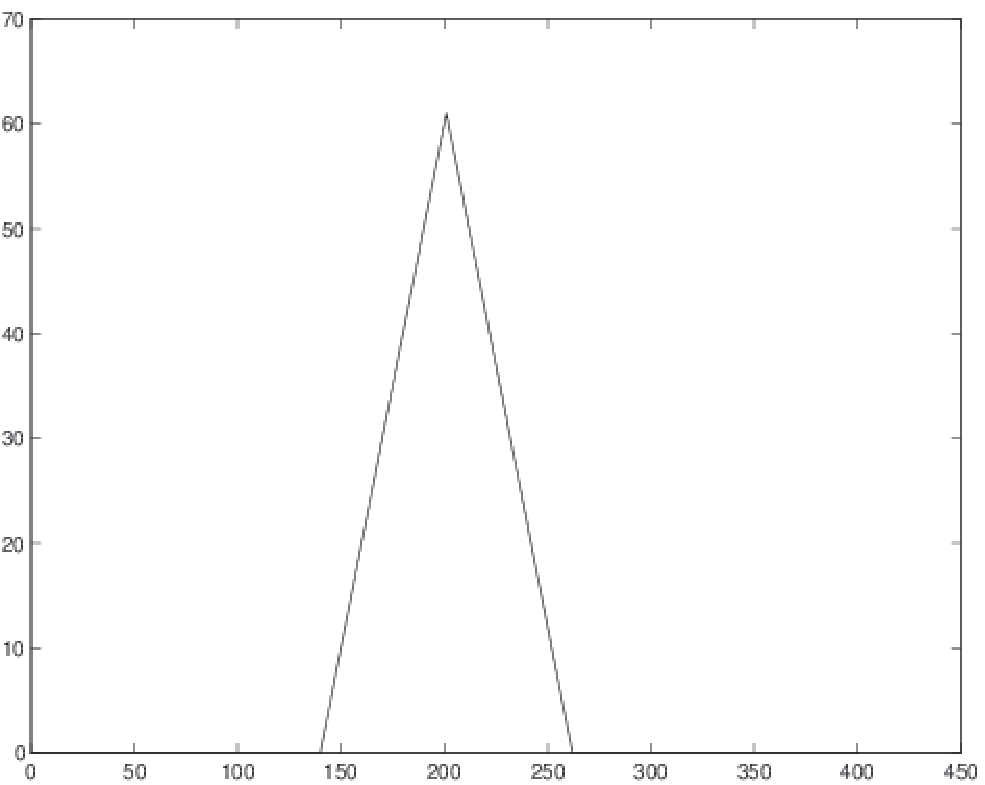
\includegraphics[scale=0.25]{convgauss2.pdf}
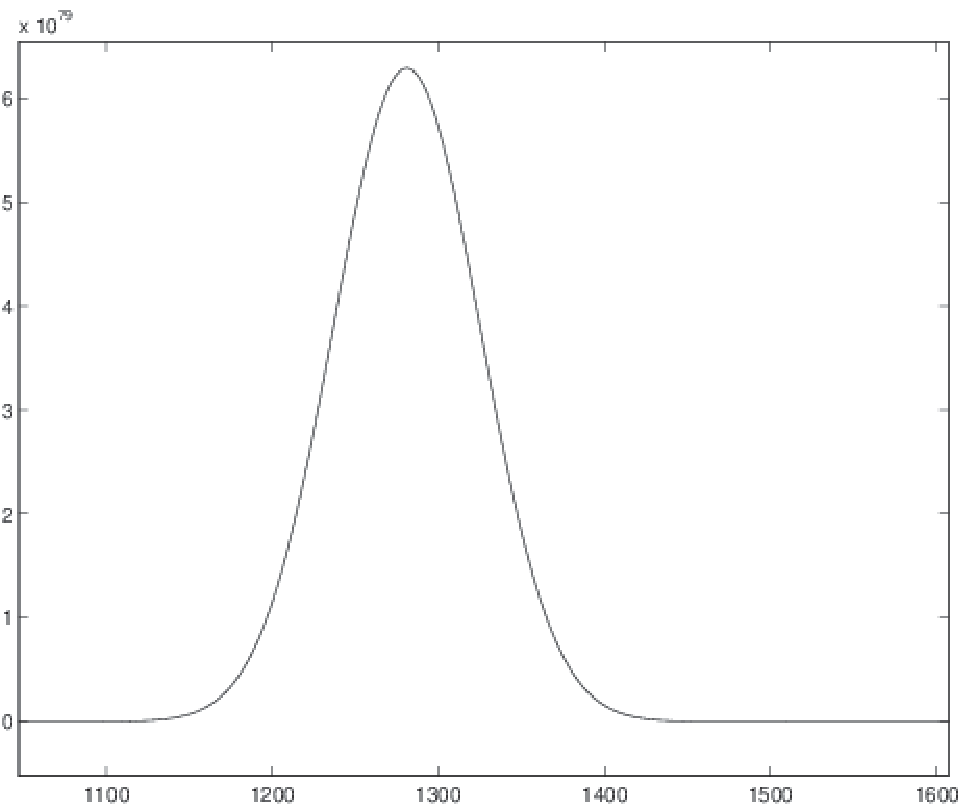
\includegraphics[scale=0.25]{convgauss3.pdf}
Fonction initiale \hspace*{1cm} Après 1 itération \hspace*{1cm} Après 6 itérations \\
\end{center}

Ce processus semble converger vers une forme gaussienne.  Un indice
supplémentaire allant dans le sens de cette supposition est que la
convolution d'une gaussienne (de moyenne $\mu_1$ et de variance
$\sigma_1^2$) par une gaussienne (de moyenne $\mu_2$ et de variance
$\sigma_2^2$) donne une gaussienne (le montrer est un bon exercice):

\begin{equation}
(\frac{e^\frac{(t-\mu_1)}{2\sigma_1^2}}{\sigma_1\sqrt{2\pi}})*
(\frac{e^\frac{(t-\mu_2)}{2\sigma_2^2}}{\sigma_2\sqrt{2\pi}})=(\frac{e^\frac{(t-(\mu_1+\mu_2))}{2(\sigma_1^2+\sigma_2^2)}}{\sqrt{2\pi(\sigma_1^2+\sigma_2^2)}})
\end{equation}

\end{example}

Au passage, une autre propriété remarquable :
\begin{equation}
  \inttotal (f*g)(t) dt=\inttotal f(t)dt \inttotal g(t)dt
\end{equation}

\subsubsection*{Illustrations}

Souvent, dans les applications de la convolution, une fonction est un
signal provenant de mesures (d'une antenne, les cours de la bourse ou
la pression atmosphérique...) et l'autre est dit { fonction noyau } (ou
simplement { noyau }), dont la forme est choisie pour modifier, analyser
ou améliorer le signal d'une façon utile.

\begin{example}
Le premier exemple (fig. \ref{fig:ex1}) montre comment on peut
approximativement { retirer le bruit } sur un signal par
convolution du signal bruité en le convoluant par une fonction
gaussienne (où on commencera à se dire { tiens, c'est simplement une
moyenne locale pondérée, un effet de lissage }).
%
\begin{figure}[h]
%
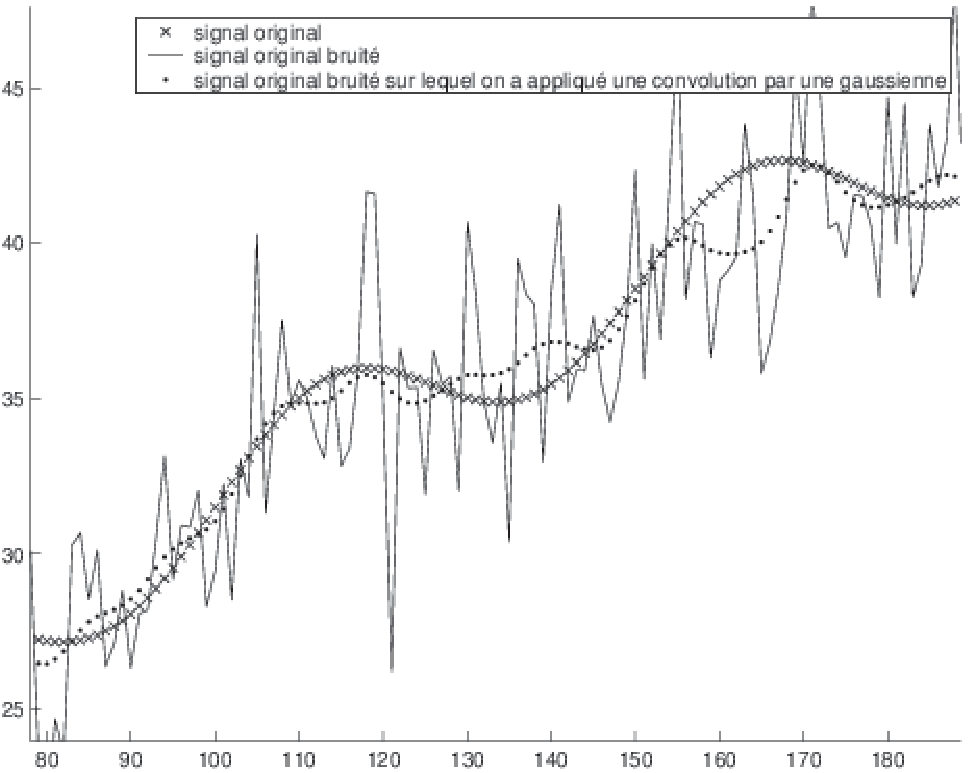
\includegraphics[scale=0.32]{con2.pdf}(a)
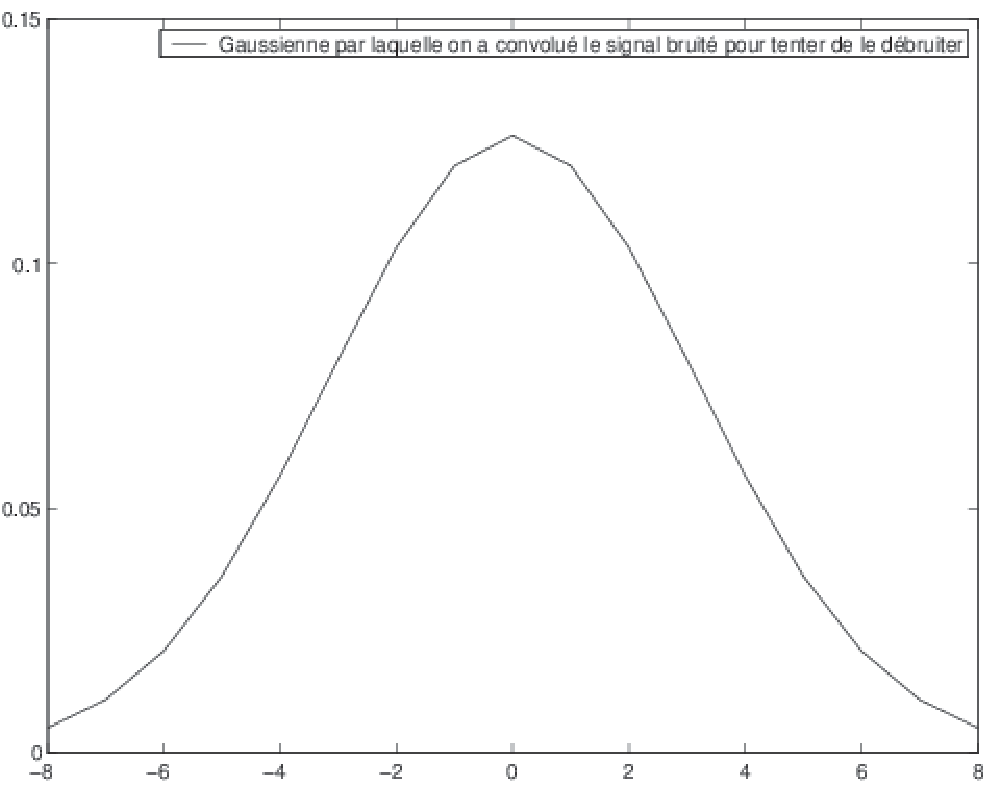
\includegraphics[scale=0.32]{con3.pdf}(b)
%
\caption{(a) Signal original : une oscillation montante, sur lequel on
a ajouté du bruit aléatoire indépendant entre instants successifs. En
convoluant ce signal bruité avec la fonction gaussienne montrée à la
figure (b), on réalise, de fait, un lissage local dans le temps,
permettant de récupérer (à peu près) le signal avant l'introduction du
bruit.}
%
\label{fig:ex1}
\end{figure}
\end{example}

\begin{example}
Le second exemple montre comment on peut détecter des discontinuités
fortes dans un signal, en convoluant le signal (on a choisi un signal
comportant des variations brusques) avec un noyau { dérivée de
gaussienne } (où on commencera à se dire { tiens, ca ressemble fort à
une sorte de calcul de dérivée }).

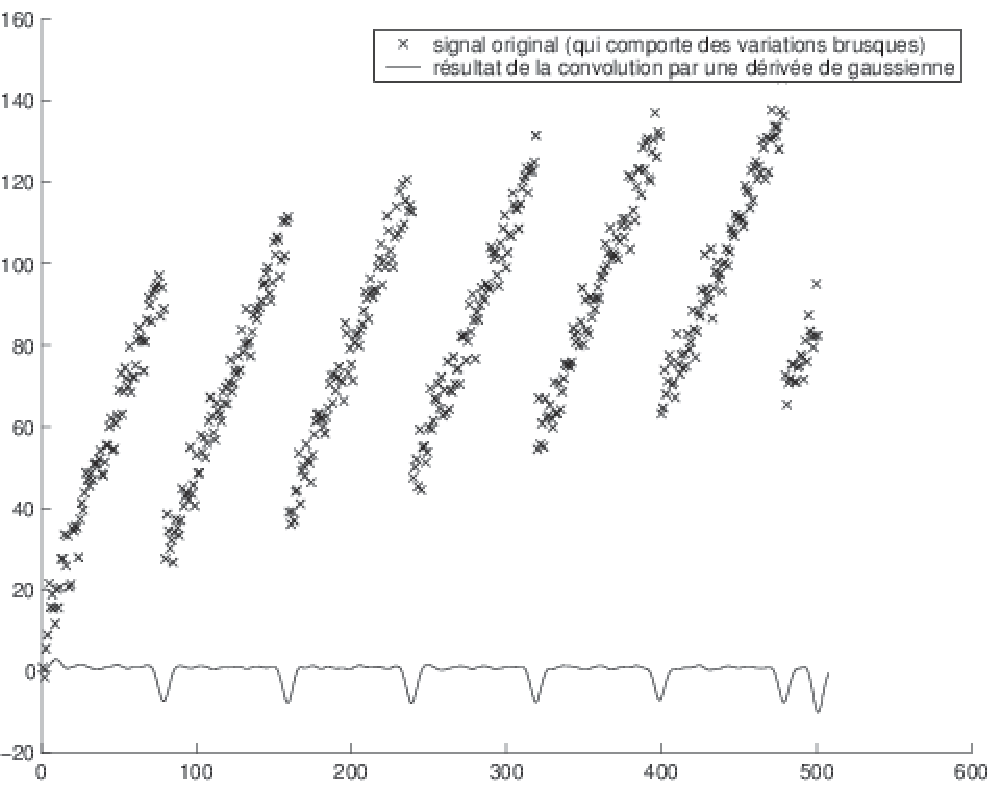
\includegraphics[scale=0.38]{con4.pdf} 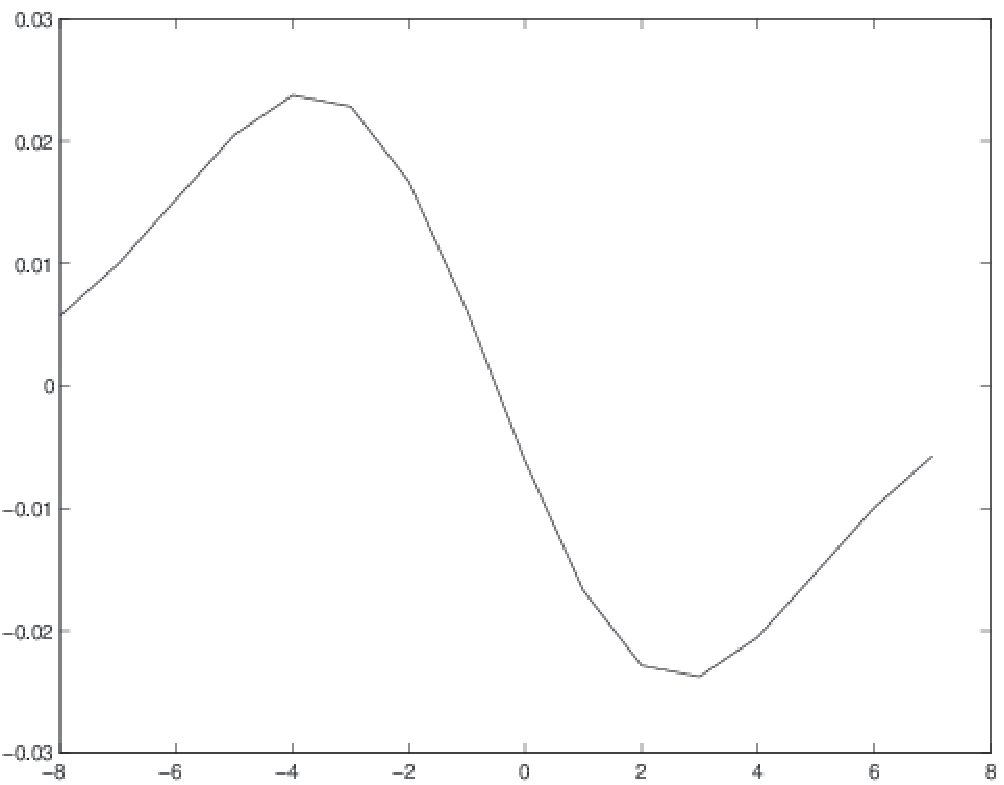
\includegraphics[scale=0.38]{con5.pdf} 
Ci-dessus à droite : fonction { dérivée de gaussienne } par laquelle on a convolué notre fonction initiale :
\end{example}

\begin{example}
En dimension 2 (cas du traitement d'image), on modélise souvent le
flou introduit par une image (par exemple en raison d'un mouvement
malheureux) comme une convolution : image floue = image nette *
operateur de flou. Remarquons au passage qu'une vision pessimiste de
notre noyau gaussien débruiteur est de dire qu'il introduit du flou
dans le signal. Une opération bien plus difficile que la convolution
mais encore plus intéressante consiste alors à trouver l'image nette à
partir de l'image floue (en particulier sans connaître l'opérateur
flouteur) : c'est une déconvolution aveugle. \\ Le même genre de
problème en dimension 1 quand un signal émis par votre téléphone
mobile veut atteindre l'antenne du réseau : il y parvient par de
multiples chemins (réflexion sur les surfaces voisines...), ce qui donne une
combinaison linéaire de diverses versions du signal émis, arrivant
avec plus ou moins de retard en fonction de la longueur de chaque
chemin. Le récepteur doit retrouver le signal d'origine, pour bien le
comprendre : voilà qui ressemble encore à notre problème de
défloutage. Une technique classique consiste à transmettre (de
l'émetteur au récepteur), de temps à autre, un signal que le
récepteur connait à l'avance : la comparaison de cette connaissance
préalable avec ce qui lui parvient lui permettra d'estimer l'opération
de { flou } causé par les chemins multiples. Il pourra utiliser
cet estimé pour déflouter la voix ou des données de l'utilisateur qui
lui parviennent les quelques secondes suivantes...
\begin{center}
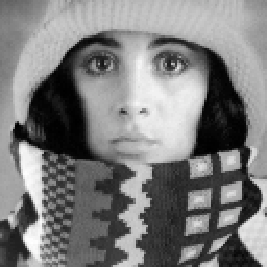
\includegraphics[scale=1]{image1.pdf} 
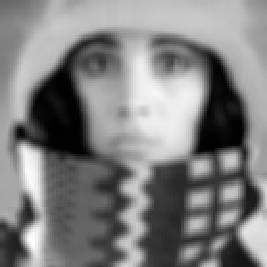
\includegraphics[scale=1]{image2.pdf}
Image originale \hspace*{2cm} Image convoluée par une gaussienne 2D \\
\end{center}
\end{example}

\subsection{Impulsion de Dirac et transformation de Fourier}
%\begin{equation*}

\begin{definition}

Considérons une fonction rectangle : 
\begin{equation}
    v(t)=
\begin{cases}
  0   & \text{si}~t \in [-\varepsilon,+\varepsilon] \\
  \frac{1}{2\varepsilon} & \text{sinon}
\end{cases}
\end{equation}
\begin{center}
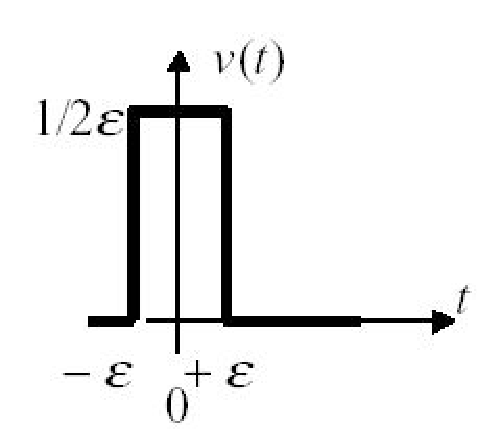
\includegraphics[scale=0.38]{dirac1.pdf} 
\end{center}

L'impulsion de Dirac est obtenue en faisant tendre $\varepsilon$ vers 0 : le rectangle est infiniment haut, infiniment étroit mais reste d'aire 1 à la limite. On aurait pu obtenir cette même limite à partir d'une fonction rectangle non nulle sur $[0,2\varepsilon]$, ou encore d'une fonction { triangle }...
où le $1$ indique l'aire et non la valeur de l'impulsion en 0 (qui est $+\infty$).
L'impulsion de Dirac est caractérisée par les propriétés suivantes :

\begin{eqnarray}
    \delta(t)=
\begin{cases}
  0   & \text{si}~t\neq0 \\
  \infty & \text{si}~t=0 
\end{cases}
\end{eqnarray}
\begin{equation}
  \inttotal \delta(t)dt~=~1
\end{equation}
\end{definition}

Le terme informel { impulsion } reste vague quant à la nature mathématique de cet objet.
Cette impulsion n'est en fait pas une \emph{fonction}, mais une \emph{distribution},
 les distributions étant une généralisation de la notion de fonction. Ces extensions sont des apports de travaux des années 1920-1950. 

L'impulsion de Dirac est notée graphiquement :
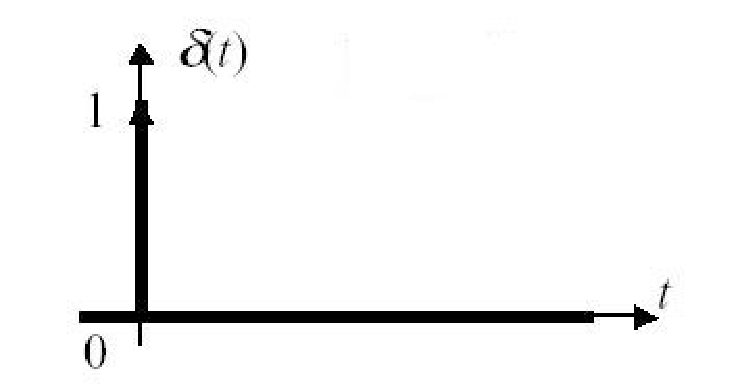
\includegraphics[scale=0.38]{dirac2.pdf} 

\begin{proposition}

\begin{equation}
 (f*\delta)(t)=\inttotal f(\tau)\delta(t-\tau)d\tau~=~f(t)
\label{proprietedirac}
\end{equation}

Autrement dit, l'impulsion de Dirac est l'élément neutre pour la convolution.
\end{proposition}

%La figure ci-dessous illustre la propriété~\ref{proprietedirac} : quand %$\varepsilon\longrightarrow~0$, le produit $f(\tau)\delta(t-\tau)$ est nul partout sauf autour %de $t=\tau$. Dans cette zone, $f(\tau)\approx f(t)$, ce qui permet de sortir $f(t)$ de %l'intégrale et de trouver le résultat~\ref{proprietedirac}.

%\begin{center}
%\input{dirac.pstex_t}
%\end{center}

Propriétés concernant l'impulsion de Dirac et la transformation de Fourier :
\begin{eqnarray}
\BF(\delta(t))~=~1 \\
\BF(1)=2\pi\delta(\om) 
\end{eqnarray}

%\end{cases}
%\end{equation*}

%Sachez aussi que l'impulsion de Dirac est la dérivée de la fonction de Heaviside (connue aussi sous le nom de fonction échelon), définie par :
%\begin{equation}
%    H(t)=
%\begin{cases}
%  1   & \text{si}~t>0 \\
%  0 & \text{sinon} 
%\end{cases}
%\end{equation}

%Remarquons qu'il y a là une extension de la notion de dérivation, puisque selon la définition usuelle, la fonction de Heaviside \footnote{La fonction paraît basique et ne méritant aucun commentaire ni même de nom particulier, jusqu'à qu'on fouille un peu de ce côté là et qu'on ouvre une boite de Pandore mathématique que l'on refermera vite ou pas (voir par ex. \emph{Analyse de Fourier et applications}, Gasquet \& Witomski pour aller plus loin.)} n'est pas dérivable en 0. Or, dans cette nouvelle dérivée, { dérivée(Heaviside)=Dirac } y compris en 0.

\subsection{Transformation de Fourier d'une fonction gaussienne}

Soit $a$ une constante strictement positive.

\begin{equation}
  \BF(e^{-at^2})=\sqrt{\frac{\pi}{a}}e^{-\frac{\om^2}{4a}}
\end{equation}


Autrement dit : la transformée de Fourier d'une gaussienne est aussi une gaussienne.

Il s'agit là d'une forme\footnote{On pourra regarder dans un second
temps la généralité de l'expression ci-dessus, pour des gaussiennes de
moyennes et variances diverses, ainsi que les constantes de
normalisation.}
%
 de fonction que l'on rencontre à chaque coin de rue,
surtout du côté des probabilités mais de manière encore plus
large. Cette propriété, qui méritera une démonstration, n'est pas
qu'esthétique - elle est par exemple exploitée dans la modulation
utilisée dans la téléphonie mobile courante.

\section{Transformée de Fourier en dimension 2}

Une application essentielle de la transformée de Fourier en dimension 2
est le traitement d'images.  La transformée existe aussi en dimension
3, utilisée pour les images { volumiques }, et également en
dimension plus élevée.

\begin{equation}
  \BF(\om_1,\om_2)=\inttotal \inttotal f(u,v)e^{-j(\om_1u+\om_2v)}~du~dv
\end{equation}
et la transformée inverse (où on omettra le cas des discontinuités) :
\begin{equation}
  f(u,v)=  \frac{1}{(2\pi)^2} \inttotal \inttotal \BF(\om_1,\om_2)e^{j(\om_1u+\om_2v)}~d\om_1~d\om_2
\end{equation}

On verra en exercice des cas où le calcul de la transformée, qui implique un calcul d'intégrale double, peut (ou pas) se formuler comme le produit de deux transformée en dimension 1.